\documentclass[11pt,a4paper,oneside]{report}
\usepackage{amsmath,amssymb,calc,ifthen}
\usepackage{float}
%\usepackage{cancel}
\usepackage[table,usenames,dvipsnames]{xcolor} % for coloured cells in tables
\usepackage{tikz}
% Allows us to click on links and references!
\usepackage{hyperref}
\usepackage{url}
\hypersetup{
colorlinks,
citecolor=black,
filecolor=black,
linkcolor=black,
urlcolor=black
}
% Nice package for plotting graphs
% See excellent guide:
% http://www.tug.org/TUGboat/tb31-1/tb97wright-pgfplots.pdf
\usetikzlibrary{plotmarks,shapes}
\usepackage{amsmath,graphicx}
\usepackage{epstopdf}
\usepackage{caption}
\usepackage{subcaption}
% highlight - useful for TODOs and similar
\usepackage{color}
\newcommand{\hilight}[1]{\colorbox{yellow}{#1}}
\newcommand\ci{\perp\!\!\!\perp} % perpendicular sign
\newcommand*\rfrac[2]{{}^{#1}\!/_{#2}} % diagonal fraction
\newcommand\SLASH{\char`\\}
\usepackage{listings}
% margin size
\usepackage[margin=1in]{geometry}
\tikzstyle{state}=[circle,thick,draw=black, align=center, minimum size=2.1cm,
inner sep=0]
\tikzstyle{vertex}=[circle,thick,draw=black]
\tikzstyle{terminal}=[rectangle,thick,draw=black]
\tikzstyle{edge} = [draw,thick]
\tikzstyle{lo} = [edge,dotted]
\tikzstyle{hi} = [edge]
\tikzstyle{trans} = [edge,->]
\definecolor{mygreen}{rgb}{0,0.6,0}
\definecolor{mygray}{rgb}{0.5,0.5,0.5}
\definecolor{mymauve}{rgb}{0.58,0,0.82}
\DeclareMathOperator*{\argmin}{arg\,min}
\DeclareMathOperator*{\argmax}{arg\,max}
\lstset{ %
backgroundcolor=\color{white}, % choose the background color; you must add
%\usepackage{color} or \usepackage{xcolor}
basicstyle=\footnotesize, % the size of the fonts that are used for the
%code
breakatwhitespace=false, % sets if automatic breaks should only happen
%at whitespace
breaklines=true, % sets automatic line breaking
captionpos=b, % sets the caption-position to bottom
commentstyle=\color{mygreen}, % comment style
deletekeywords={...}, % if you want to delete keywords from the
%given language
escapeinside={\%*}{*)}, % if you want to add LaTeX within your code
extendedchars=true, % lets you use non-ASCII characters; for
%8-bits encodings only, does not work with UTF-8
frame=single, % adds a frame around the code
keepspaces=true, % keeps spaces in text, useful for keeping
%indentation of code (possibly needs columns=flexible)
keywordstyle=\color{blue}, % keyword style
language=Octave, % the language of the code
morekeywords={*,...}, % if you want to add more keywords to the set
numbers=left, % where to put the line-numbers; possible
%values are (none, left, right)
numbersep=5pt, % how far the line-numbers are from the code
numberstyle=\tiny\color{mygray}, % the style that is used for the line-numbers
rulecolor=\color{black}, % if not set, the frame-color may be changed
%on line-breaks within not-black text (e.g. comments (green here))
showspaces=false, % show spaces everywhere adding particular
%underscores; it overrides 'showstringspaces'
showstringspaces=false, % underline spaces within strings only
showtabs=false, % show tabs within strings adding particular
%underscores
stepnumber=2, % the step between two line-numbers. If it's
%1, each line will be numbered
stringstyle=\color{mymauve}, % string literal style
tabsize=2, % sets default tabsize to 2 spaces
title=\lstname % show the filename of files included with
%\lstinputlisting; also try caption instead of title
}
\title{Computational Modelling for Biomedical Imaging - Coursework 1}
\author{
Razvan Valentin Marinescu\\
Student Number: 14060166\\
\texttt{razvan.marinescu.14@ucl.ac.uk}
}
\begin{document}
\belowdisplayskip=12pt plus 3pt minus 9pt
\belowdisplayshortskip=7pt plus 3pt minus 4pt
\maketitle{}

\section*{Q1.1.1}



%Think about the quality of the fit you obtain above.  First, eyeball the fit 
%to the data by comparing the predictions from the model with your fitted 
%parameters to the actual measurements, as in the lectures. 

From eyeballing the data in fig. \ref{q111} we notice that the fit is very poor, especially for the 3 entries where the b-value is 0, having a $\Delta S > 7 * 10^5$. The other entries don't fit the data well either.

%Then, is the final 
%value of RESNORM above the kind of value for the sum of square differences we 
%expect?  

The final value of RESNORM (1.2242e+12) is clearly above the kind of value we would normally expect. The fit is poor probably because the search strategy got stuck in a local minima.

%The standard deviation of the noise on each measurement of this data 
%set is somewhere in the range 5000-­‐6000.  Given that, what would you expect a 
%typical value of RESNORM to be? 
 

The expected value of RESNORM would be given by the formula:
$$E\left[\sum_{i=1}^{33} (X_i - \bar{X}_i)^2\right] = E\left[\sum_{i=1}^{33} \sigma_i^2\right] = 33 * \sigma^2 $$
Since sigma is between 5000-6000 this means that $ 8.25*10^8 < RESNORM < 1.188 * 10^9$.

%Are the parameter values sensible given the 
%quantities they represent?	

Some of the parameter values we obtain are not sensible. For example, the value of $f$ is negative, meaning that we have negative intra-axonal diffusion, which is not physically possible. The value of S0 is also really high, when in fact it should be around $1.1 * 10^5$. 


\section*{Q1.1.2}
%% TODO: insert picture (maybe)


I did the following transformations:
\begin{itemize}
 \item $S0 \to S0^2$
 \item $d \to d^2$
 \item $f \to (1+e^{-f})^{-1}$ (sigmoid)
\end{itemize}
This time the algorithm converges to the following parameters: $S0 = 1.132129e+05, d=1.534e-03 f=0.575, \theta=-1.03,  \phi=-0.11$ with a RESNORM of 1.33e+09. These parameter values are realistic and give us a RESNORM that is around 1000 times smaller. Note that we this time the starting parameters were changed to more realistic values ($S0 = 1.5e+05, d=3e-03 f=0.5, \theta=0,  \phi=0$). The reason we gett better parameters and RESNORM is because we introduced the transformations that keep the parameters within reasonable limits and because we used a better starting position.

\section*{Q1.1.3}
Running the same procedure for gaussian-distributed starting points and for three different pixels gives us the following parameters:
\begin{center}
\begin{tabular}{c | c | c | c | c | c | c}
Voxel & S0 & d & f & $\theta$ & $\phi$ & GlobalMinCounter(out of 100)\\
\hline
(52,62,25) & 1.132e+05 & 1.534e+03 & 0.575 & 2.10 & 6.17 & 89\\
(63,40,18) & 1.121e+05 & 1.829e+03 & 0.5125 & 1.19 & 5.43 & 83\\
(50,64,23) & 1.214e-05 & 7.208e-04 & 0.1955 & 5.05 & 5.02 & 87\\
\end{tabular}
\end{center}

GlobalMinCounter represents the number of times the global minimum was found was found. We are quite confident that those are the global minimums, since we made sure that the covariance of the gaussian distribution from which we sample the starting position is large enough to cover a wide area of the space. If we consider the probability $p$ of finding the global minimum in one run, then after $k$ runs the probability of \textbf{not} having found the global minimum would be $(1-p)^k$ where $k$ is the number of runs. Then, the minimum number of runs in order to be 95\% confident that we will find the global minimum is $\argmin_{k} 0.05 > (1-p)^k$. Since $p \approx 0.86$ then $k = 2$, meaning that 2 runs are enough to be 95\% confident.

\section*{Q1.1.4}

The maps for $S0$, $d$, $f$, $RESNORM$ and the fibre direction $n$ are shown in figures \ref{q114-S0}, \ref{q114-D}, \ref{q114-F}, \ref{q114-RESNORM} and \ref{q114-fbDir} respectively. 

\section*{Q1.1.5}

I implemented the DTI model and used the following mappings to get to the parameters of the BallStick model:
\begin{enumerate}
 \item $d = mean(D)$, $f = 0.5 ( |\lambda_1'- \lambda_2'| + |\lambda_1'- \lambda_3'| + |\lambda_2'- \lambda_3'|) $ where $\lambda_i' = \lambda_i/(\lambda_1 + \lambda_2 + \lambda_3)$ for $i \in 1..3$
 \item $d = tr(D)/3$, $f$ as above
 \item $d = max(D)$,  $f = 0.5 ( (\lambda_1'- \lambda_2')^2 + (\lambda_1'- \lambda_3')^2 + (\lambda_2'- \lambda_3')^2) $, for $\lambda_i'$ as above
\end{enumerate}

The most efficient was method 1, for which the global minimum was found in approximatively 93/100 runs. The parameters I got using method 1 are:$S0=1.13184e+05$, $Dxx=0.00125$, $Dxy=-0.00013$, $Dxz=-0.00053$, $Dyy=0.00043$, $Dyz=0.00011$ and $Dzz=0.000782$ with a $RESNORM=1.4458e+09$.



\section*{Q1.1.6}

The computation time for \texttt{fmincon} is around 9x slower when compared to \texttt{fminunc} (averaged over 100 trials, \texttt{fmincon}=6.68sec, \texttt{fminunc}=56.28sec). Nevertheless, the global minimum is almost always found by both functions (87/100 runs). The parameters and $RESNORM$ it converges to are the same as in Q1.1.2.

\section*{Q1.1.7}

For 10 runs using gaussian distributed starting positions, the time it takes without gradient is 11 seconds while this gets reduced to 7 seconds if the gradient is used. 


\section*{Q1.1.8}

\section*{Q1.2.1}

The histogram of $p(x|A)$ along with the $2\sigma$ and 95\% ranges are shown for parameters $S0$, $d$ and $f$ in figures \ref{q121-p1}, \ref{q121-p2} and \ref{q121-p3} respectively. These have been computed for the voxel (52,62,25). Parameter estimates for various other voxels are given in table \ref{q121tab}. A better visualisation\footnote{plot contains two other methods apart from parametric bootstrap: MCMC and Laplace} of the parameter intervals for $S0$, $d$ and $f$  is given in figures \ref{q123-p1}, \ref{q123-p2}, \ref{q123-p3}. The $2\sigma$ and 95\% confidence ranges all agree with each other and have roughly the same mean. In table \ref{q121tab} all voxels have similar ranges for $S0$, however voxel (70,64,14) has different ranges for 
$d$ and $f$, probably because it is a CSF or gray matter voxel. In figures \ref{q123-p1}, \ref{q123-p2}, \ref{q123-p3} we notice that the $2\sigma$ range is always smaller than the 95\% confidence interval, for all parameters. 

\section*{Q1.2.2}

 The $2\sigma$ and 95\% confidence ranges for MCMC are given in figures \ref{q123-p1}, \ref{q123-p2}, \ref{q123-p3}. Ranges reported by MCMC have the same mean as the ranges generated by the parametric bootstrap, but they are larger, suggesting that MCMC covers a larger parameter space.

\section*{Q1.2.3}

I only managed to implement Laplace's method. 

\section*{Q1.3.1}

The parameters that I found are: $S0=0.9231$, $d=1.1355e-09$, $f=0.49$, $\theta=4.704$, $\phi=0.038$ with a $RESNORM=3.8681$. The predicted signal is plotted against the measurements in figure \ref{q131}. The parameters have been found by applying \texttt{fmincon} for reveral rounds of 100 times, with random starting positions sampled from a gaussian distribution with mean $\mu$. Parameter vector $\mu$ was updated at each iteration with the global minimum found in the previous round.

\section*{Q1.3.2}
For fitting these models I decided to switch to \texttt{fminunc} because it is faster and slightly more efficient at finding the global minimum. For the Zeppelin-Stick model I actually made implementations with both functions and realised that for the same starting position, \texttt{fminunc} was converging to better parameters and $RESNORM$ than \texttt{fmincon}. The fit for these models can be visualised in figures \ref{q132-DiffTensor}, \ref{q132-ZeppStick} and \ref{q132-ZeppStickTort}. The best model was the Zeppelin-Stick, with a $RESNORM=1.1784$, followed by Zeppelin-Stick with tortuosity, Ball-stick and DTI having $RESNORMS$ of 2.1337, 3.8681 and 20.5832 respectively. The main reason the Zeppelin-Stick model outperforms the others is because it is more general than ZeppelinStick with tortuosity and Ball-Stick, having more parameters. It is therefore expected to perform at least as good as the others.

% The parameters they converge to are given in table \ref{q132-tab}.

\section*{Q1.3.5}


\section*{Q1.3.3}

\begin{center}
\begin{tabular}{c | c | c | c | c}
& Zeppelin-Stick & Zeppelin-Stick Tort & Ball-Stick & Diffusion Tensor\\
\hline
AIC & 750 & 1345 & 2427 & 12878\\
BIC & 785 & 1375 & 2452 & 12913\\
\end{tabular}
\end{center}

The AIC and BIC scores show that the Zeppelin-Stick model is the one performing best (having the lowest scores), followed by Zeppelin-Stick with tortuosity, Ball-Stick and DTI. AIC and BIC rankings are consistent across the models. 


\section*{Q1.4.1}

\section*{Q1.4.2}



\section*{Images}

\section*{Q1.1.1}

\begin{figure}[H]
\centering
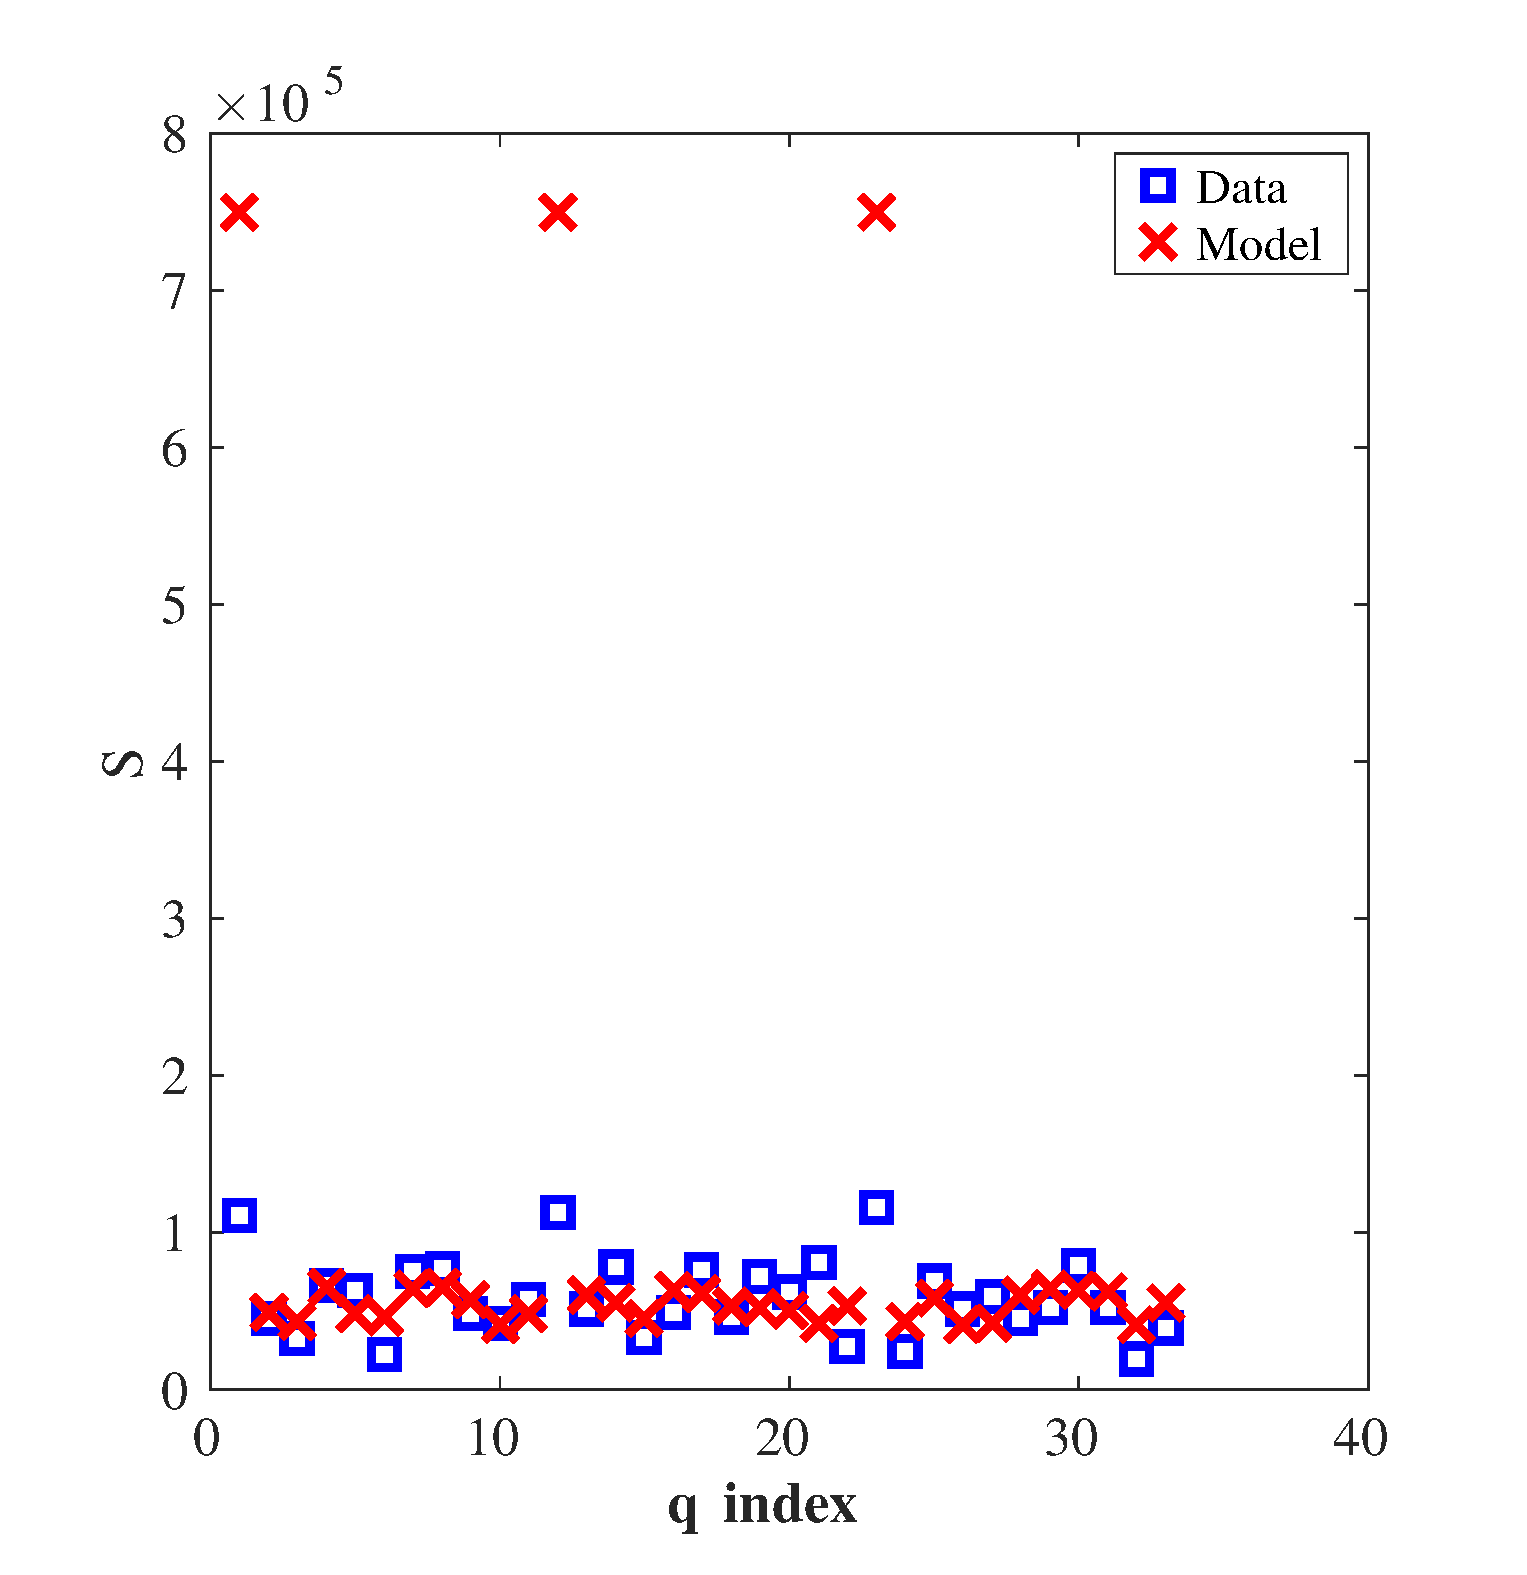
\includegraphics[scale=0.5]{figures/q1/q111.eps}
\caption{Estimated of the Ball-Stick model for the voxel at position $(52,62,25)$}
\label{q111}
\end{figure}

\section*{Q1.1.4}

\begin{figure}[H]
  \centering
  \begin{subfigure}[b]{0.5\textwidth}
    %trim=l b r t
      \centering
    \includegraphics[scale=1]{figures/q1/q114-S0.eps}
    \caption{$S0$ map}
    \label{q114-S0}
  \end{subfigure}%
  ~
  \begin{subfigure}[b]{0.5\textwidth}
    %trim=l b r t
      \centering
    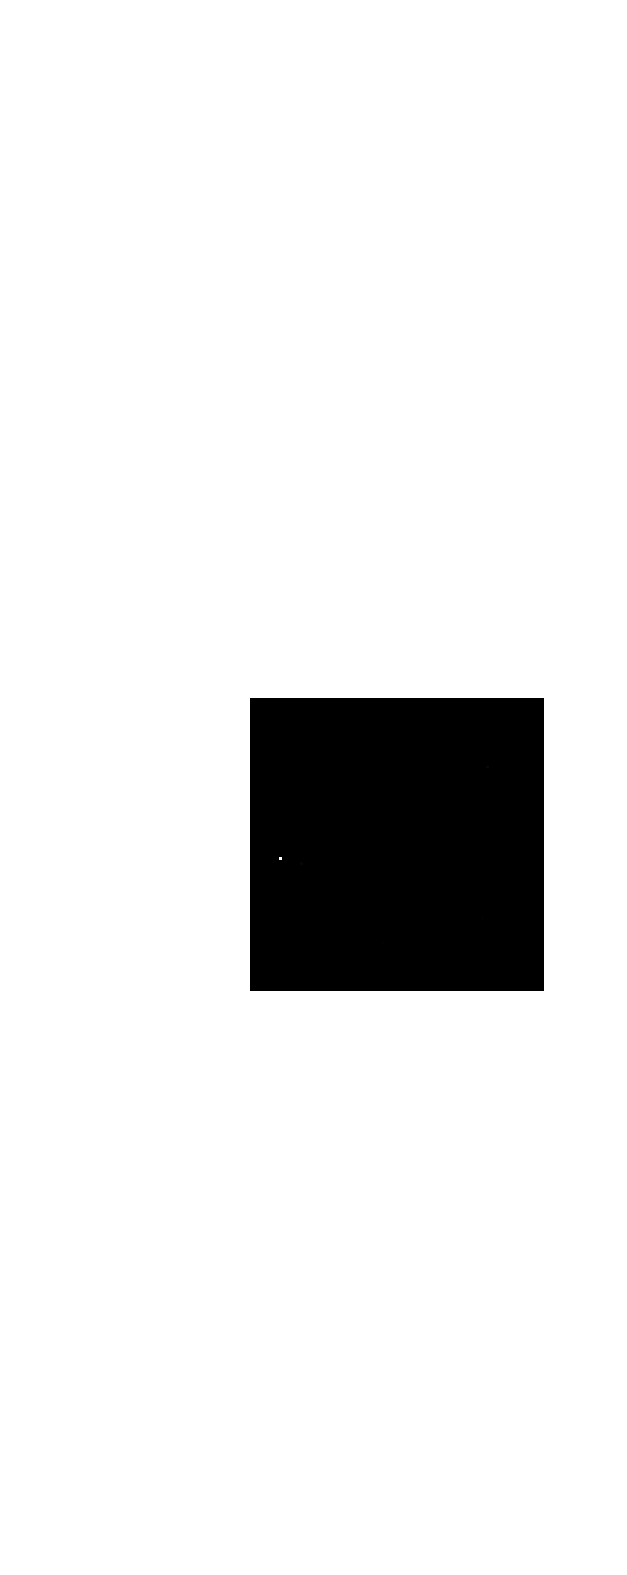
\includegraphics[scale=1]{figures/q1/q114-D.eps}
    \caption{$D$ map}
    \label{q114-D}
  \end{subfigure}%
  \caption{}

\end{figure}

\begin{figure}[H]
  \centering
  \begin{subfigure}[b]{0.5\textwidth}
    %trim=l b r t
      \centering
    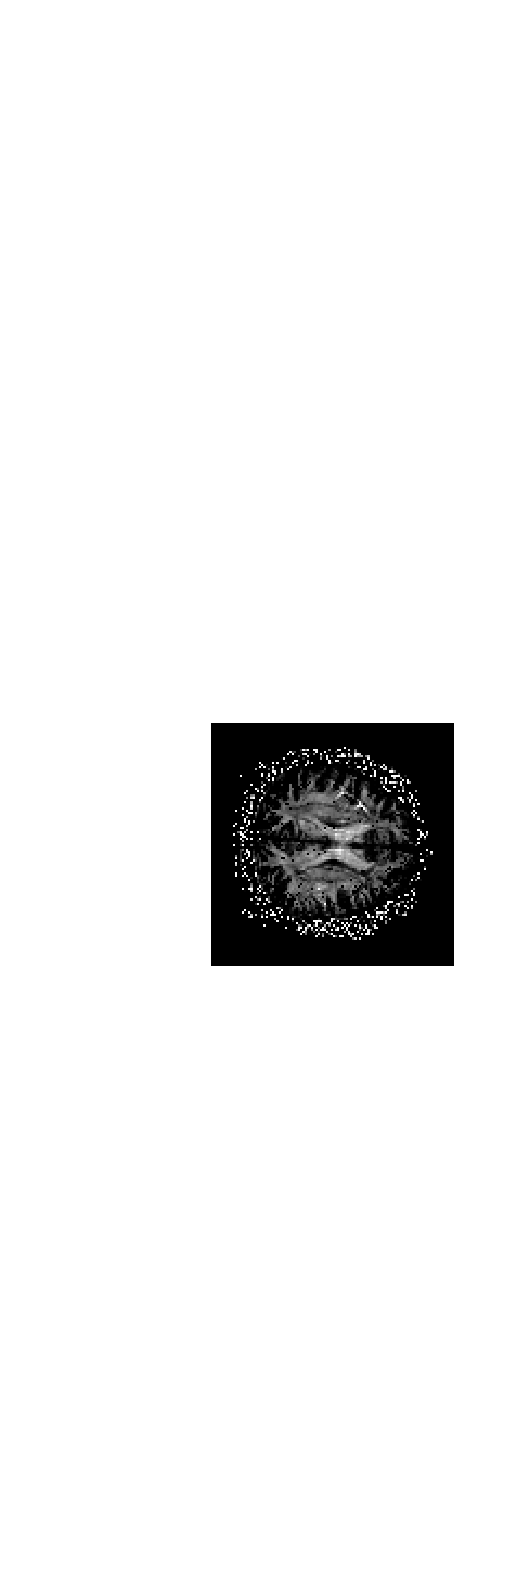
\includegraphics[scale=1]{figures/q1/q114-F.eps}
    \caption{$F$ map}
    \label{q114-F}
  \end{subfigure}%
  ~
  \begin{subfigure}[b]{0.5\textwidth}
    %trim=l b r t
      \centering
    \includegraphics[scale=1]{figures/q1/q114-RESNORM.eps}
    \caption{$RESNORM$ map}
    \label{q114-RESNORM}
  \end{subfigure}%
  \caption{}

\end{figure}

\begin{figure}[H]
      \centering
    \includegraphics[scale=1]{figures/q1/q114-fbDir.eps}
    \caption{Fibre direction map}
    \label{q114-fbDir}
\end{figure}

\section*{Q1.2.1}

\begin{figure}[H]
      \centering
    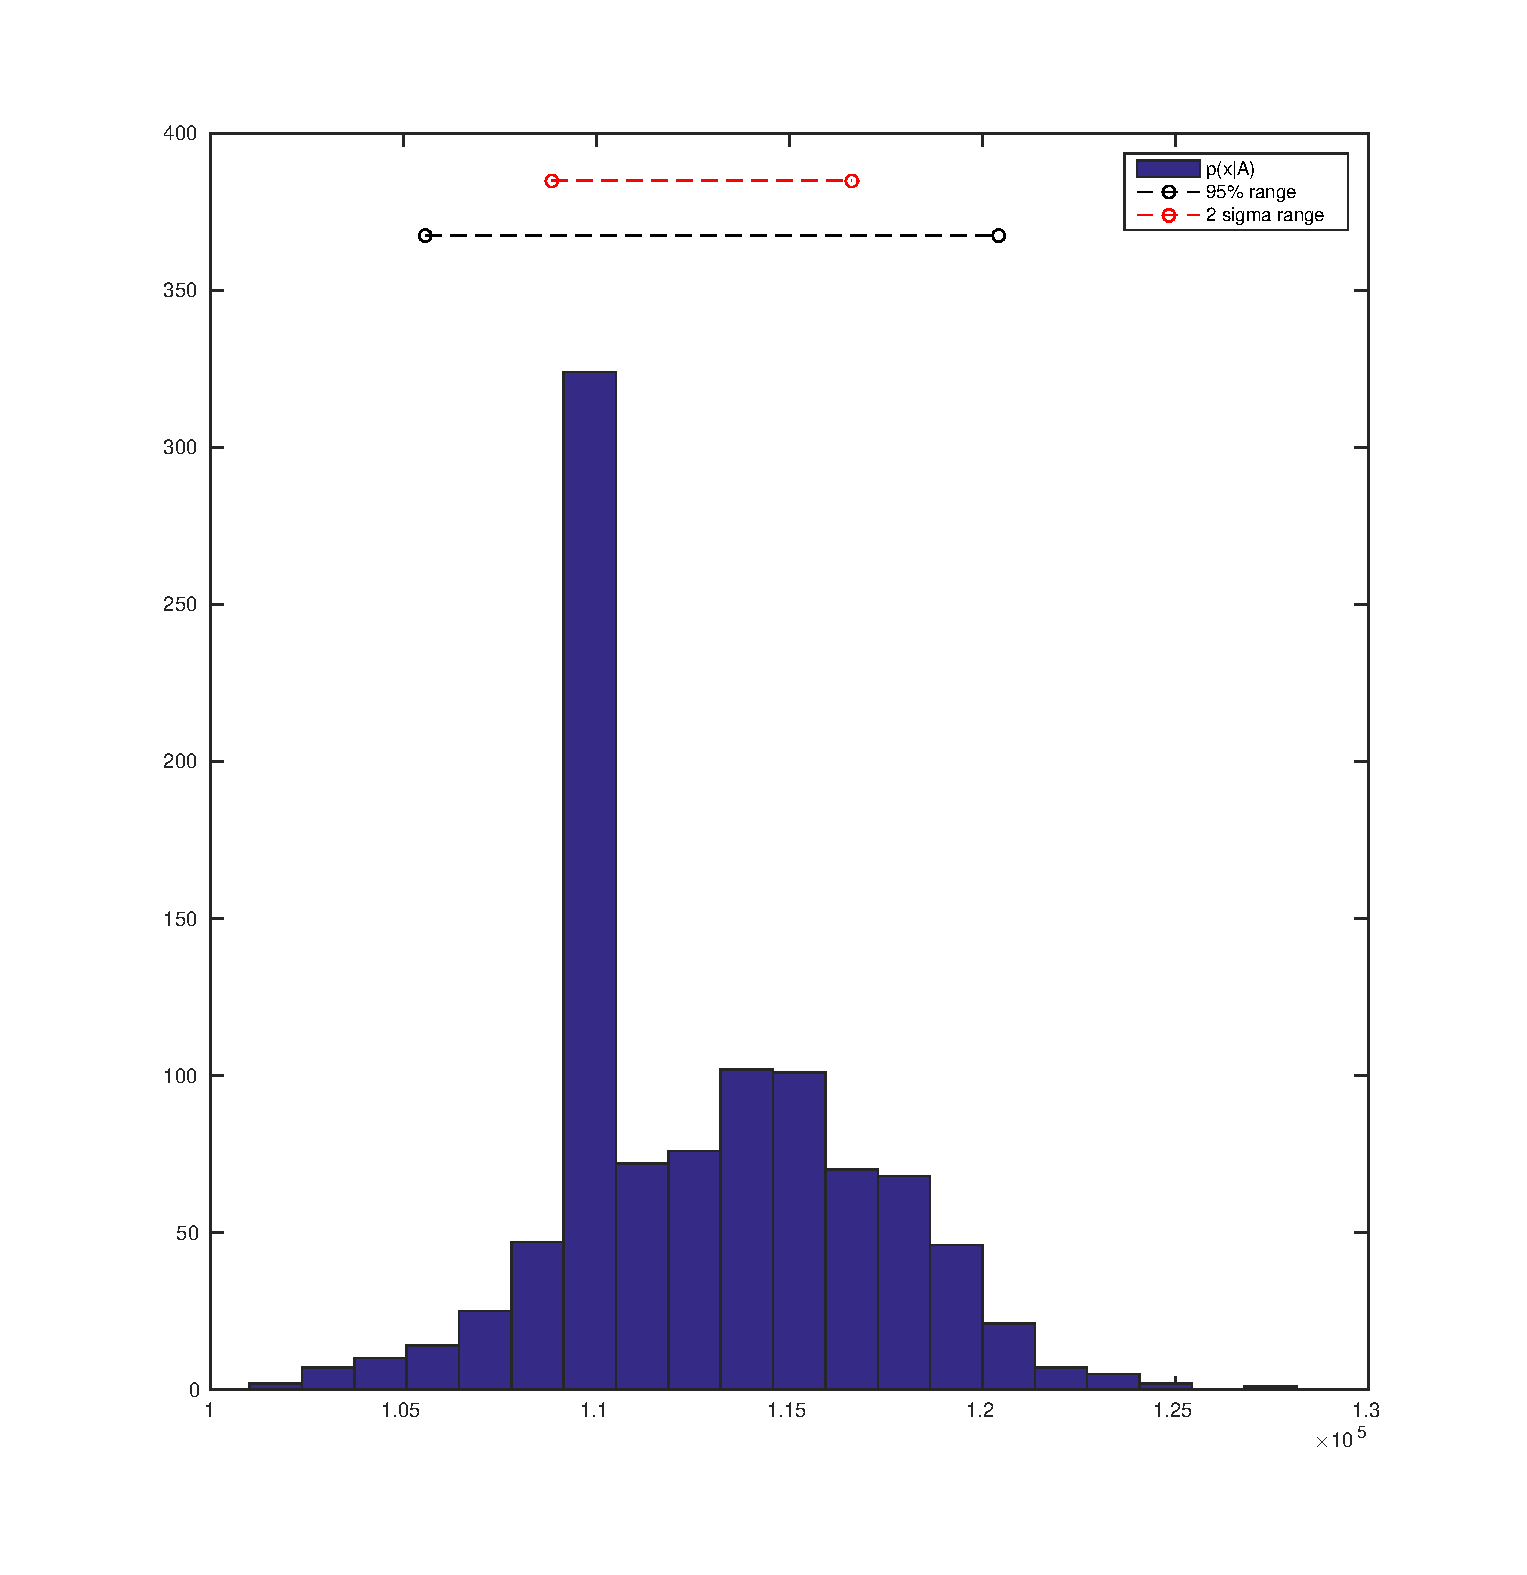
\includegraphics[scale=1]{figures/q2/q121-p1.eps}
    \caption{Parametric bootstrap for $S0$ using voxel (52,62,25)}
    \label{q121-p1}
\end{figure}

\begin{figure}[H]
      \centering
    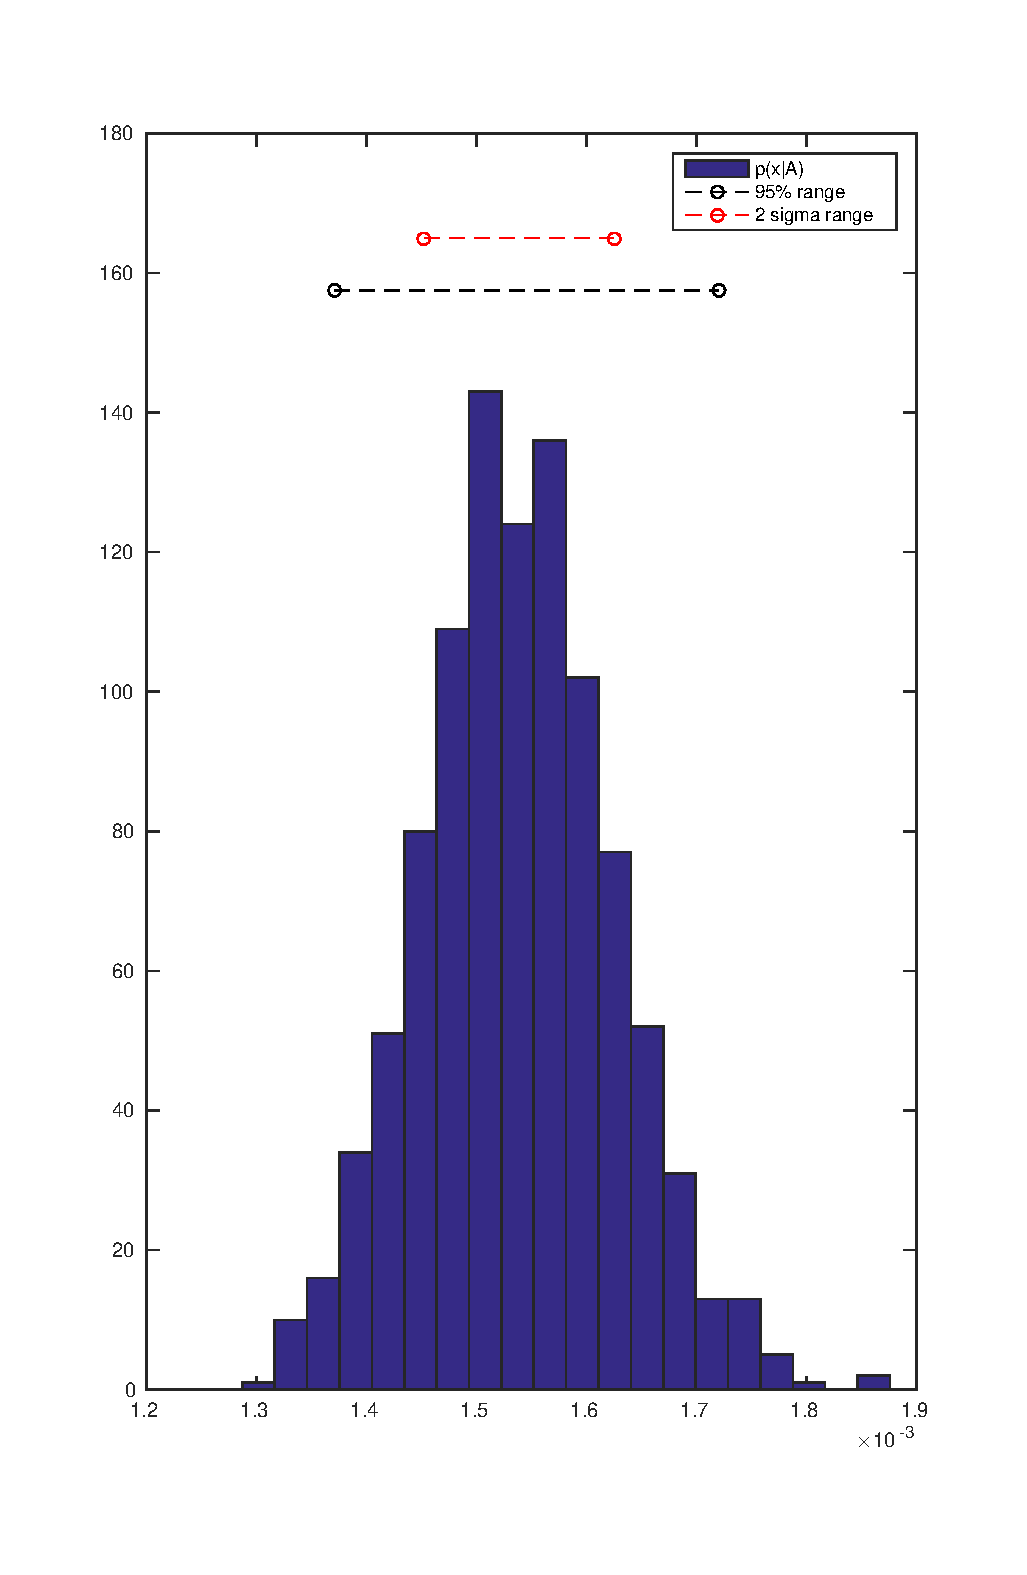
\includegraphics[scale=1]{figures/q2/q121-p2.eps}
    \caption{Parametric bootstrap for $d$ using voxel (52,62,25)}
    \label{q121-p2}
\end{figure}

\begin{figure}[H]
      \centering
    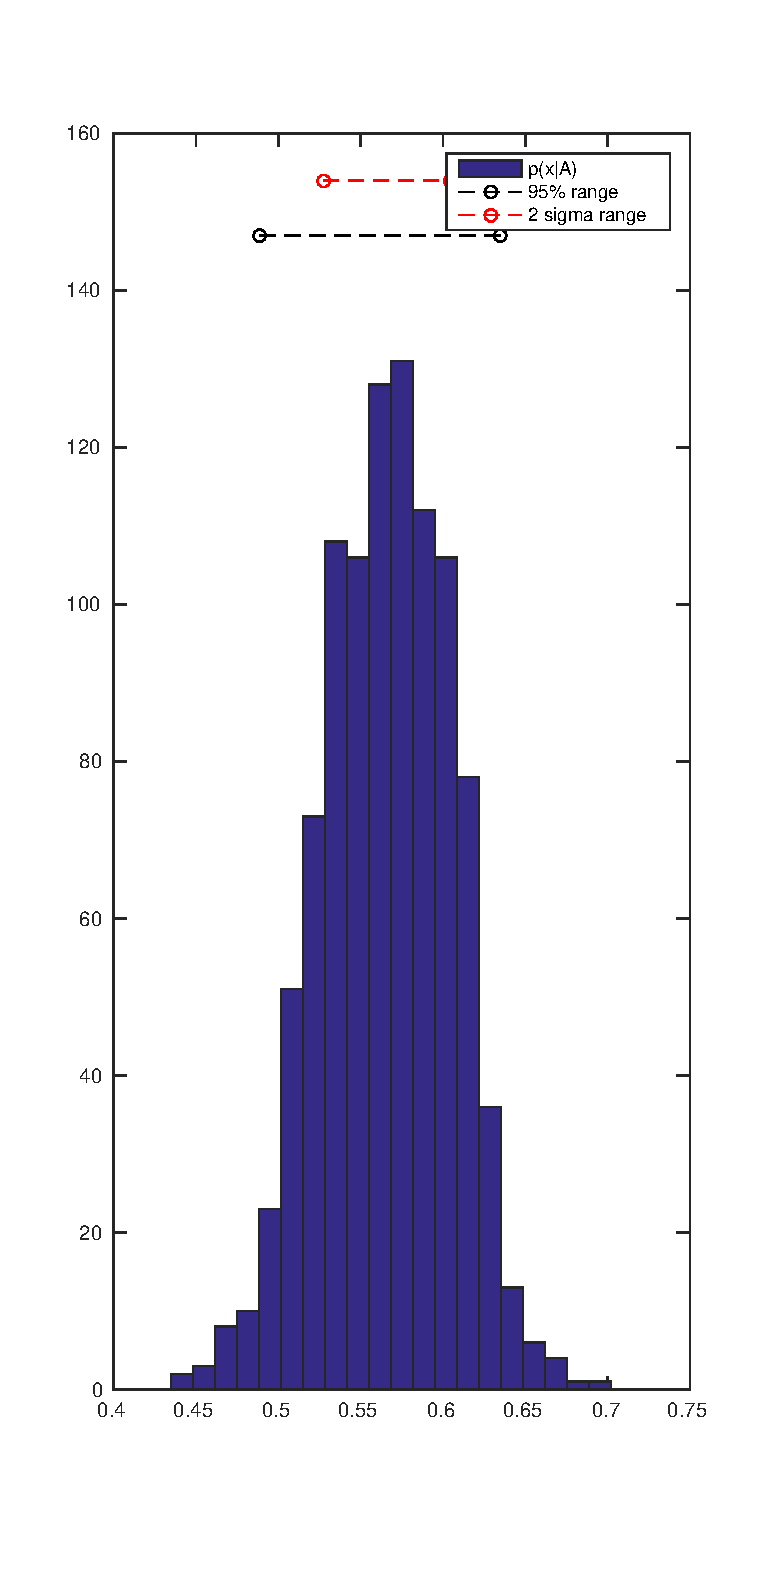
\includegraphics[scale=1]{figures/q2/q121-p3.eps}
    \caption{Parametric bootstrap for $f$ using voxel (52,62,25)}
    \label{q121-p3}
\end{figure}

\begin{table}[H]
\begin{center}
\begin{tabular}{c | c | c | c | c | c | c}
\multicolumn{7}{c}{2-sigma ranges}\\
 Voxel & \multicolumn{2}{c|}{$S0$} & \multicolumn{2}{c|}{$d$} & \multicolumn{2}{c}{$f$}\\ 
 \hline
 (52,62,25) & 1.088e+05 & 1.166e+05 & 1.452e-03 & 1.624e-03 & 0.527 & 0.604\\
 (63,40,18) & 1.017e+05 & 1.229e+05 & 1.026e-03 & 1.397e-03 & 0.136 & 0.326\\
 (70,64,14) & 1.022e+05 & 1.112e+05 & 7.584e-04 & 8.928e-04 & 0.078 & 0.185\\
  \hline
  \multicolumn{7}{c}{}\\
  \multicolumn{7}{c}{95\% confidence intervals}\\
 (52,62,25) & 1.055e+05 & 1.204e+05 & 1.370e-03 & 1.719e-03 & 0.488 & 0.634\\
 (63,40,18) & 0.918e+05 & 1.330e+05 & 0.870e-03 & 1.608e-03 & 0.000 & 0.404\\
 (70,64,14) & 0.976e+05 & 1.152e+05 & 6.888e-04 & 9.507e-04 & 0.000 & 0.231\\
\end{tabular}
\caption{2-sigma and 95\% confidence intervals for voxel (52,62,25) using Parametric bootstrap}
\label{q121tab}
\end{center}
\end{table}


\section*{Q1.2.2 \& Q1.2.3}

\begin{figure}[H]
      \centering
    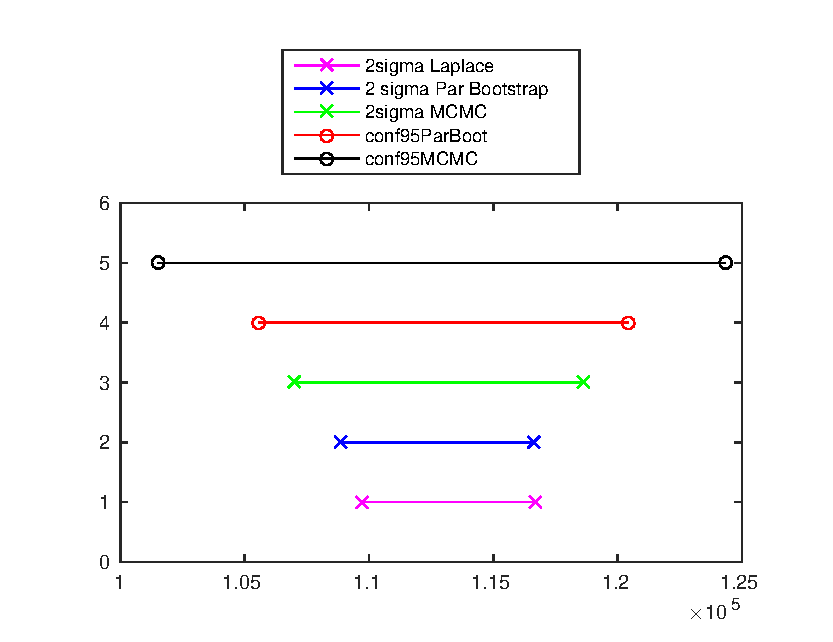
\includegraphics[scale=1]{figures/q2/q123-p1.eps}
    \caption{$2\sigma$ and 95\% confidence intervals on parameter $S0$ using three different methods: parametric bootstrap, MCMC and Laplace. Voxel used was (52,62,25) }
    \label{q123-p1}
\end{figure}

\begin{figure}[H]
      \centering
    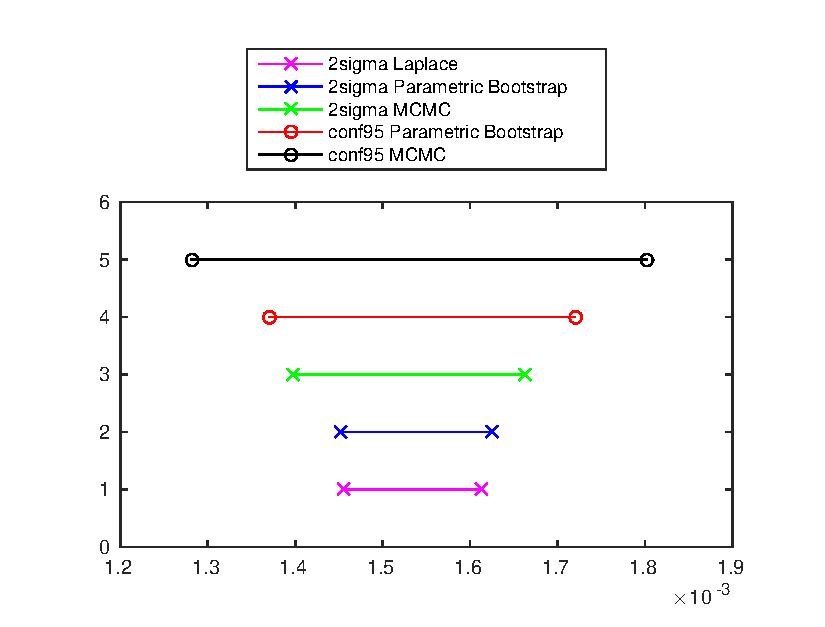
\includegraphics[scale=1]{figures/q2/q123-p2.eps}
    \caption{$2\sigma$ and 95\% confidence intervals on parameter $d$ using three different methods: parametric bootstrap, MCMC and Laplace. Voxel used was (52,62,25) }
    \label{q123-p2}
\end{figure}

\begin{figure}[H]
      \centering
    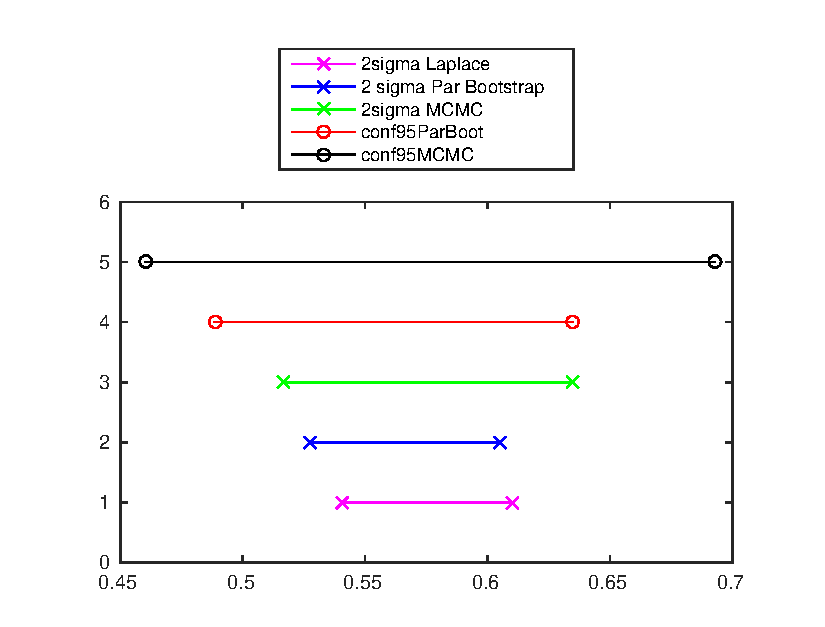
\includegraphics[scale=1]{figures/q2/q123-p3.eps}
    \caption{$2\sigma$ and 95\% confidence intervals on parameter $f$ using three different methods: parametric bootstrap, MCMC and Laplace. Voxel used was (52,62,25) }
    \label{q123-p3}
\end{figure}

\section*{Q1.3.1}

\begin{figure}[H]
%\hspace{-3em}
\centering
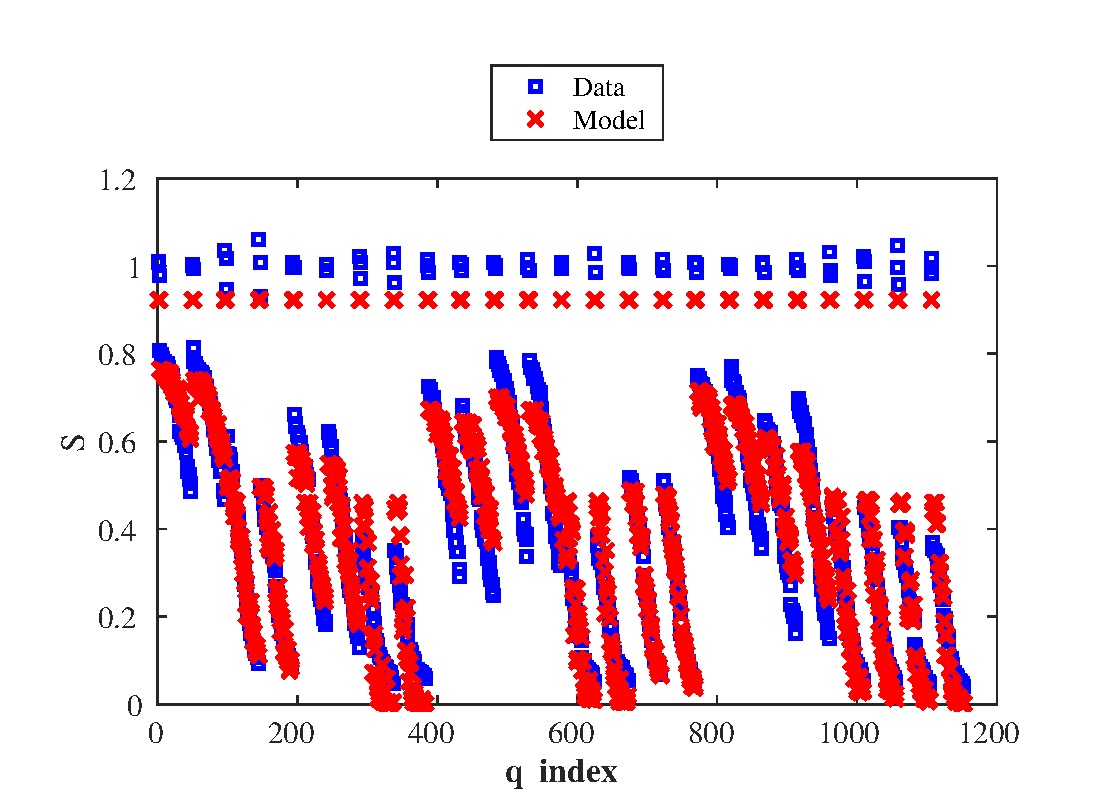
\includegraphics[scale=0.8]{figures/q3/q131.eps}
\caption{Estimated fit for the Ball-Stick model for the given voxel. RESNORM=3.8681}
\label{q131}
\end{figure}

\section*{Q1.3.2}

\begin{figure}[H]
%\hspace{-3em}
\centering
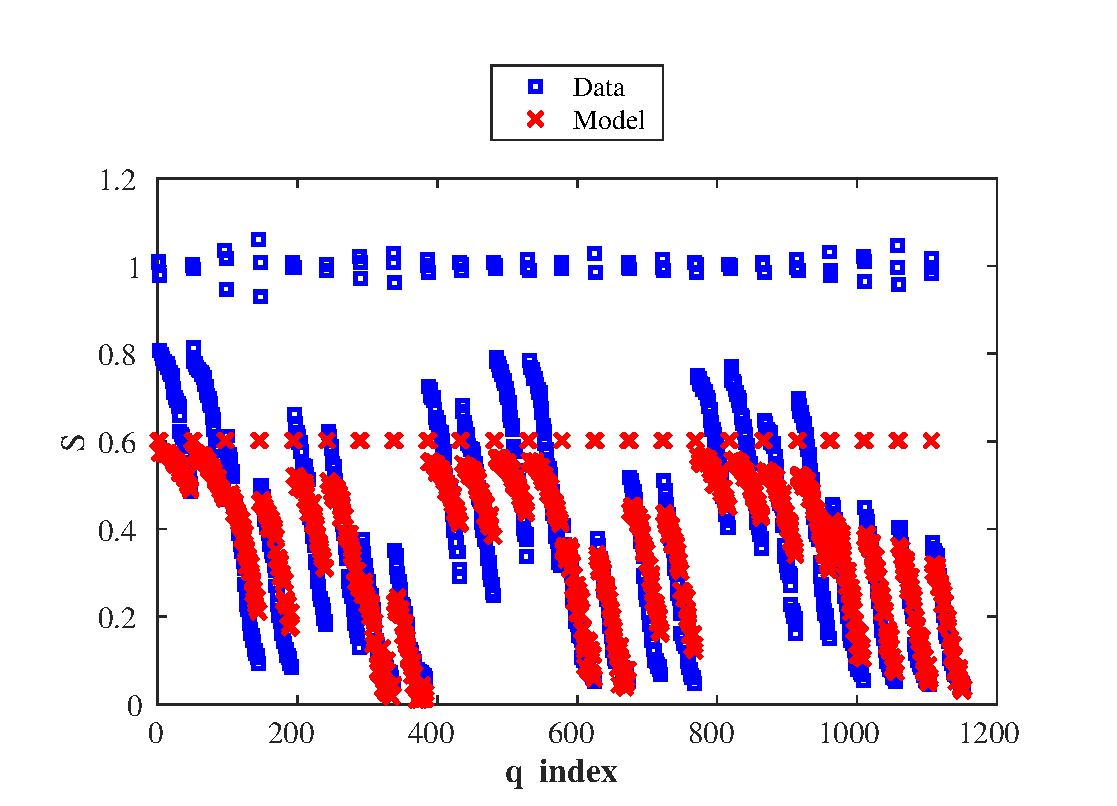
\includegraphics[scale=0.8]{figures/q3/q132-DiffTensor.eps}
\caption{Estimated fit for Diffusion Tensor model for the given voxel. RESNORM=20.5832}
\label{q132-DiffTensor}
\end{figure}

\begin{figure}[H]
%\hspace{-3em}
\centering
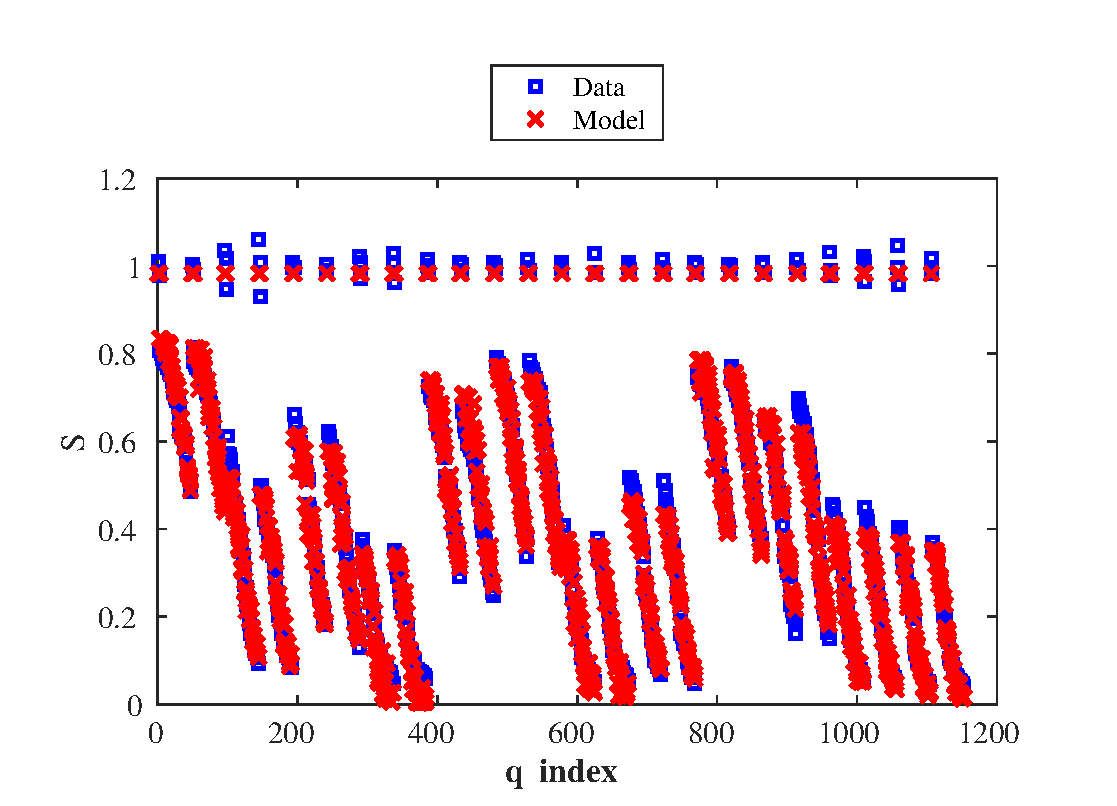
\includegraphics[scale=0.8]{figures/q3/q132-ZeppStick.eps}
\caption{Estimated fit for Zeppelin-Stick model for the given voxel. RESNORM=1.1784}
\label{q132-ZeppStick}
\end{figure}

\begin{figure}[H]
%\hspace{-3em}
\centering
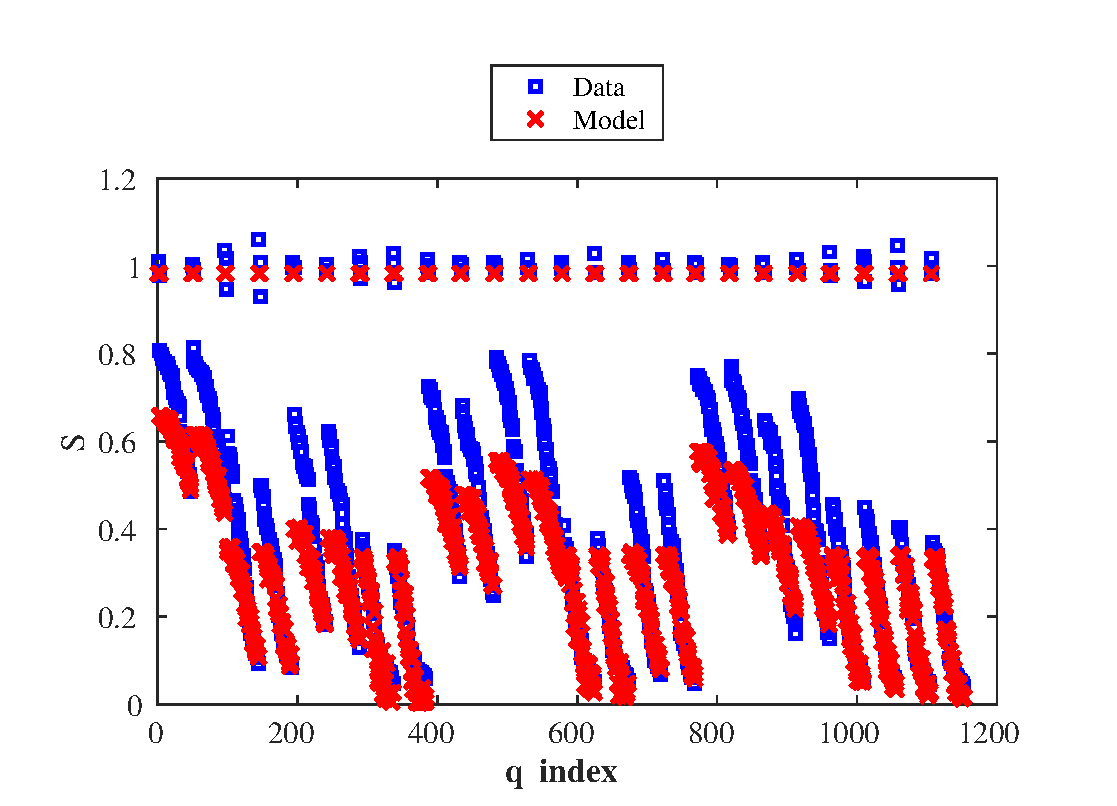
\includegraphics[scale=0.8]{figures/q3/q132-ZeppStickTort.eps}
\caption{Estimated fit for Zeppelin-Stick with tortuosity model for the given voxel. RESNORM=2.1337}
\label{q132-ZeppStickTort}
\end{figure}

% \begin{table}[H]
% \begin{center}
% \begin{tabular}{c | c }
% \multicolumn{7}{c}{2-sigma ranges}\\
%  \hline
%   Zeppelin-Stick & $S0=0.9816$, $d=0.9816$, $f=0.345$, $\theta=4.68$, $\phi=3.16$, $\lambda_1=2.87e-09$, $\lambda_2=6.843e-10$\\
%   Ball-Stick & $S0=0.9231$, $d=1.1355e-09$, $f=0.49$, $\theta=4.704$, $\phi=0.038$,$RESNORM=3.8681$\\
% \end{tabular}
% \caption{Glaobal minimum parameters for the Zeppelin-Stick, Zeppelin-Stick with tortuosity, Ball-Stick and DTI models.}
% \label{q132-tab}
% \end{center}
% \end{table}

\end{document}





















